\begin{figure}[htbp] 
\centering 
	\subfigure[\textit{F}-DEA$^{*}$]
	{
		\label{fig:dtlz110fdeastarfigure}
		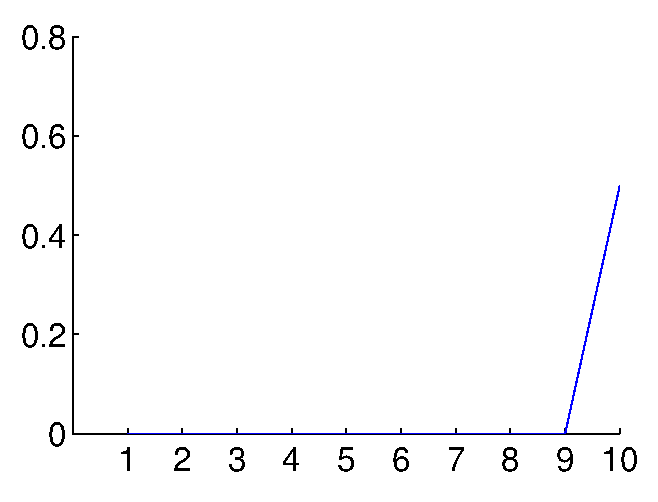
\includegraphics[width=0.20\textwidth]{figures/experiments/comparison/fdeawithoutclusterdtlz1_10.eps}
	}	
	\hspace{0em}	
	\subfigure[\textit{F}-DEA$^{\#}$]
	{
		\label{fig:dtlz110fdeahashfigure}
		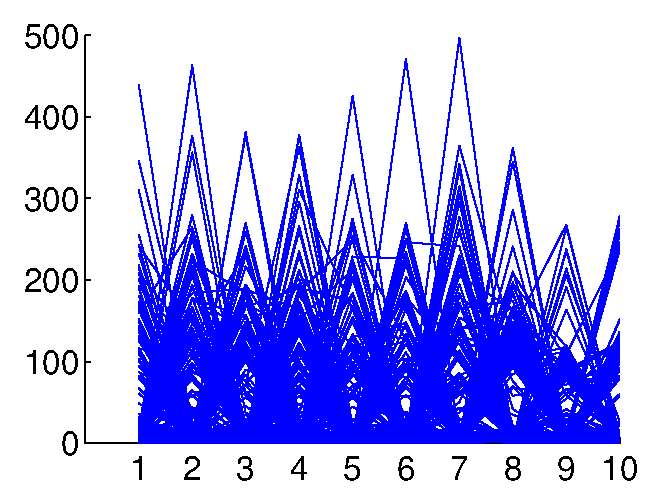
\includegraphics[width=0.20\textwidth]{figures/experiments/comparison/fdeaparetodtlz1_10.eps}
	}	
	\hspace{0em}
	\subfigure[Basic \textit{F}-DEA]
	{
		\label{fig:dtlz110fdeafigure}
		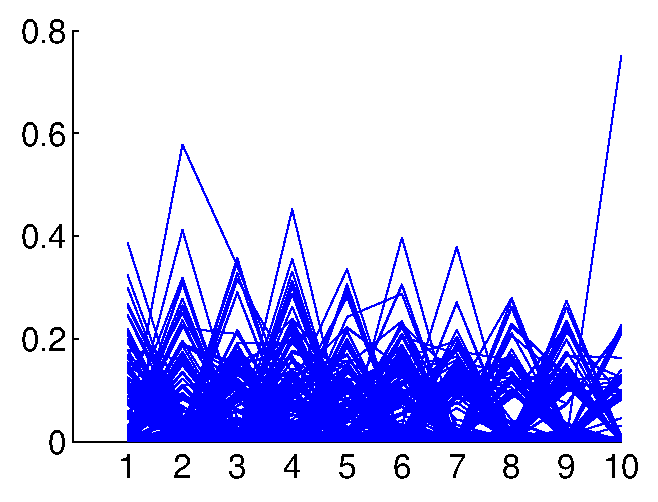
\includegraphics[width=0.20\textwidth]{figures/experiments/comparison/fdeagausdtlz1_10.eps}
	}
\caption{Parallel coordinate plots of variants of $F$-DEA on $10-$ objective DTLZ1 problem. }
\label{fig:dtlz110figure}
\end{figure}